\section*{Лекция 8 (07.04.2022)}


5. $f : \R ^ m \to \R$

Как иначе част. произв.

\[
    \frac{\partial f}{\partial x_j}(a) = \lim_{t \to 0} \frac{f(a + t b_j) - f(a)}{t}
\] --- частные производные


\quad

\tikzset{every picture/.style={line width=0.75pt}} %set default line width to 0.75pt        

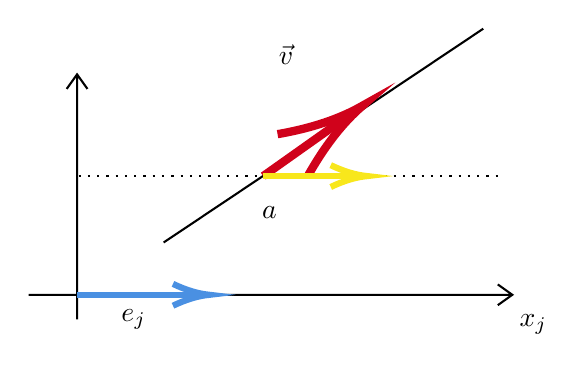
\begin{tikzpicture}[x=0.75pt,y=0.75pt,yscale=-1,xscale=1]
%uncomment if require: \path (0,300); %set diagram left start at 0, and has height of 300

%Shape: Axis 2D [id:dp9687964262664879] 
\draw  (49,178.2) -- (282,178.2)(72.3,72) -- (72.3,190) (275,173.2) -- (282,178.2) -- (275,183.2) (67.3,79) -- (72.3,72) -- (77.3,79)  ;
%Straight Lines [id:da9894643901800455] 
\draw    (114,153) -- (268,50) ;
%Straight Lines [id:da7026880280506494] 
\draw [color={rgb, 255:red, 208; green, 2; blue, 27 }  ,draw opacity=1 ][line width=3]    (162,121) -- (205.92,89.89) ;
\draw [shift={(210,87)}, rotate = 144.69] [color={rgb, 255:red, 208; green, 2; blue, 27 }  ,draw opacity=1 ][line width=3]    (41.53,-12.5) .. controls (26.41,-5.31) and (12.57,-1.14) .. (0,0) .. controls (12.57,1.14) and (26.41,5.31) .. (41.53,12.5)   ;
%Straight Lines [id:da07635776933551464] 
\draw [color={rgb, 255:red, 74; green, 144; blue, 226 }  ,draw opacity=1 ][line width=2.25]    (72.3,178.2) -- (132,178.2) ;
\draw [shift={(136,178.2)}, rotate = 180] [color={rgb, 255:red, 74; green, 144; blue, 226 }  ,draw opacity=1 ][line width=2.25]    (17.49,-5.26) .. controls (11.12,-2.23) and (5.29,-0.48) .. (0,0) .. controls (5.29,0.48) and (11.12,2.23) .. (17.49,5.26)   ;
%Straight Lines [id:da964758185077272] 
\draw  [dash pattern={on 0.84pt off 2.51pt}]  (73,121) -- (275,121) ;
%Straight Lines [id:da24048133962313678] 
\draw [color={rgb, 255:red, 248; green, 231; blue, 28 }  ,draw opacity=1 ][line width=2.25]    (162,121) -- (208,121) ;
\draw [shift={(212,121)}, rotate = 180] [color={rgb, 255:red, 248; green, 231; blue, 28 }  ,draw opacity=1 ][line width=2.25]    (17.49,-5.26) .. controls (11.12,-2.23) and (5.29,-0.48) .. (0,0) .. controls (5.29,0.48) and (11.12,2.23) .. (17.49,5.26)   ;

% Text Node
\draw (168,56.4) node [anchor=north west][inner sep=0.75pt]    {$\vec{v}$};
% Text Node
\draw (160,134.4) node [anchor=north west][inner sep=0.75pt]    {$a$};
% Text Node
\draw (92.15,183.6) node [anchor=north west][inner sep=0.75pt]    {$e_{j}$};
% Text Node
\draw (284,186.4) node [anchor=north west][inner sep=0.75pt]    {$x_{j}$};


\end{tikzpicture}

\quad

\begin{definition}
    \[
        \frac{\partial f}{\partial \vec{v}}(a) = \lim_{t \to 0} \frac{f(a + tv) - f(a)}{t}
        \text{ --- производная вдоль вектора $\vec{v}$}
    \] 
\end{definition}

    если $\abs{\vec{v}} = 1 \hence $ производная по направлению $\vec{v}$


    Пусть $f$ дифф. в $(\cdot) a \hence \exists df(a), \exists \frac{\partial f}{\partial x_j}(a)$
    
    $\vec{v} = v_1 e_1 + ... v_m e_m \hence f(a + t(v_1 e_1 + ... v_n e_n)) = f(a) + \sum t v_j \underbrace{df(a) e_j}_{\frac{\partial f}{\partial x_j}(a)} + o(t)$  \\ (раскрыли по линейности)


    $f(a) + t \langle \nabla f(a), \vec{v} \rangle + o(t) \hence \underbrace{\frac{\partial f}{\partial \vec{v}}}_{\text{изменение $f$ вдоль $\vec{v}$}} (a) = \langle \nabla f(a), \vec{v} \rangle$


    $max_{\abs{\vec{v}} = 1} \langle \nabla f(a), \vec{v} \rangle = \abs{\nabla f(a)}$ достигается на $\vec{v} = \frac{\nabla f(a)}{\abs{\nabla f(a)}}$ --- экстремальное свойство градиента



\tikzset{every picture/.style={line width=0.75pt}} %set default line width to 0.75pt        

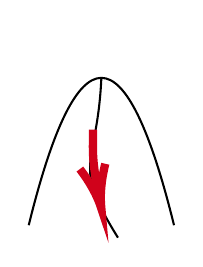
\begin{tikzpicture}[x=0.75pt,y=0.75pt,yscale=-1,xscale=1]
%uncomment if require: \path (0,300); %set diagram left start at 0, and has height of 300

%Shape: Parabola [id:dp4302115536680866] 
\draw   (278,227) .. controls (301.33,132.33) and (324.67,132.33) .. (348,227) ;
%Curve Lines [id:da24889808956414328] 
\draw    (313,156) .. controls (311,200) and (298,196) .. (321,233) ;
%Curve Lines [id:da9311162491050265] 
\draw [color={rgb, 255:red, 208; green, 2; blue, 27 }  ,draw opacity=1 ][line width=3]    (309,181) .. controls (309,191.23) and (308.14,194.54) .. (312.04,214.26) ;
\draw [shift={(313,219)}, rotate = 258.23] [color={rgb, 255:red, 208; green, 2; blue, 27 }  ,draw opacity=1 ][line width=3]    (20.77,-6.25) .. controls (13.2,-2.65) and (6.28,-0.57) .. (0,0) .. controls (6.28,0.57) and (13.2,2.66) .. (20.77,6.25)   ;




\end{tikzpicture}


\quad

\begin{remark}

    $f : X \to Y$, $\frac{\partial f}{\partial \vec{v}}(a) = \lim \frac{f(a + t \vec{v}) - f(a)}{t}$

    Если $f$ дифф. в $(\cdot) a \hence \frac{\partial f(a)}{\partial \vec{v}} = df(a) \vec{v} \in Y$
\end{remark}



\subsection{Теорема о конечном приращении (теорема Лагранжа о среднем)}

\begin{theorem}
    $U \text{ --- откр.} \subset X, a, h \in X, f : U \to Y, [a, a + h] \subset U, f$ дифф. на $(a, a + h)$



\tikzset{every picture/.style={line width=0.75pt}} %set default line width to 0.75pt        

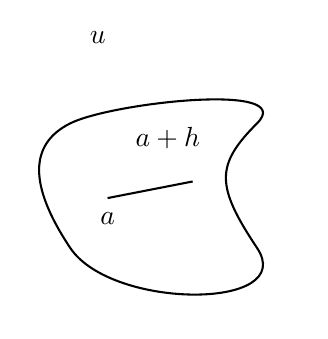
\begin{tikzpicture}[x=0.75pt,y=0.75pt,yscale=-1,xscale=1]
%uncomment if require: \path (0,300); %set diagram left start at 0, and has height of 300

%Shape: Polygon Curved [id:ds9693110599256342] 
\draw   (242,125) .. controls (262,115) and (352,105) .. (332,125) .. controls (312,145) and (312,155) .. (332,185) .. controls (352,215) and (262,215) .. (242,185) .. controls (222,155) and (222,135) .. (242,125) -- cycle ;
%Straight Lines [id:da9230232026238654] 
\draw    (260,161) -- (301,153) ;

% Text Node
\draw (250,79.4) node [anchor=north west][inner sep=0.75pt]    {$u$};
% Text Node
\draw (255,166.4) node [anchor=north west][inner sep=0.75pt]    {$a$};
% Text Node
\draw (272,125.4) node [anchor=north west][inner sep=0.75pt]    {$a+h$};


\end{tikzpicture}



$[a, b] = \{ a \lambda + b (1 - \lambda) | \lambda \in [0, 1]\}$


$\hence \norm{f(a+h) - f(a)}_Y \leqslant \underbrace{\sup_{\xi \in (a, a + h)} \norm {df(\xi)}_{L(X, Y)}}_{sup_{\theta \in (0, 1) \norm{df(a + \theta h)}}} \cdot \norm{h}_X$
\end{theorem}

\begin{remark}

\begin{enumerate}

    \item  $f : \R \to \R, f(a + h) - f(a) = f'(a + \theta h) h $   --- теорема Лагранжа
    \item В многомерье на равенство расчитывать нельзя. 
    $f : \R \to \R ^ 2, f(t) = (\cos t, \sin t) \hence f(0) = f(2\pi), df(\theta) \neq 0, \forall \theta$
\end{enumerate}
   
\end{remark}

\begin{proof}
    $M = \sup_{\xi \in (a, a + h)} \norm{df(\xi)} < \infty$

    Проверим, что $\forall [\xi^-, \xi^+] \subset (a, a + h) \hence \norm{f(\xi^+) - f(\xi^-)} \leqslant M \norm{\xi^+ - \xi^-}$

    От противного $\exists \varepsilon_0 \exists [\xi_1^-, \xi_1^+ : \norm{f(\xi_1^+) - f(\xi_1^-)} \geqslant (M + \varepsilon_0) \norm{\xi_1^+ - \xi_1^-}] \hence $ либо для пары $[ \xi_1, \frac{\xi_1^- + \xi_1^+}{2}] , [ \frac{\xi_1^- + \xi_1^+}{2}, \xi_1^+]$ выполнено такое же нерв-во 

    $[\xi_2^-, \xi_2^+]$, ..., $[\xi_n^-, \xi_n^+]$

    $\cap [\xi_n^-, \xi_n^+] = \{ \xi^* \}$ 

    $\{ \xi^* \} \in (a, a + h) \hence \norm{df(\xi^*)} \leqslant M$




\tikzset{every picture/.style={line width=0.75pt}} %set default line width to 0.75pt        

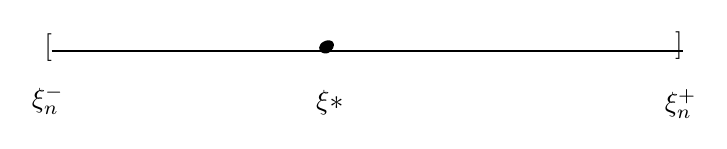
\begin{tikzpicture}[x=0.75pt,y=0.75pt,yscale=-1,xscale=1]
%uncomment if require: \path (0,300); %set diagram left start at 0, and has height of 300

%Straight Lines [id:da39346125885318417] 
\draw    (100,108) -- (404,108) ;
%Shape: Free Drawing [id:dp6639686754544865] 
\draw  [color={rgb, 255:red, 0; green, 0; blue, 0 }  ][line width=3] [line join = round][line cap = round] (233,107) .. controls (230.75,107) and (232.43,105.43) .. (233,106) .. controls (233.94,106.94) and (231.94,107.94) .. (231,107) .. controls (230.15,106.15) and (232.86,104.62) .. (234,105) .. controls (234.89,105.3) and (232,107.94) .. (232,107) ;

% Text Node
\draw (95,98.4) node [anchor=north west][inner sep=0.75pt]    {$[$};
% Text Node
\draw (399,97.4) node [anchor=north west][inner sep=0.75pt]    {$]$};
% Text Node
\draw (89,123.4) node [anchor=north west][inner sep=0.75pt]    {$\xi _{n}^{-}$};
% Text Node
\draw (394,125.4) node [anchor=north west][inner sep=0.75pt]    {$\xi _{n}^{+}$};
% Text Node
\draw (226,125.4) node [anchor=north west][inner sep=0.75pt]    {$\xi *$};


\end{tikzpicture}


$f(\xi_n^-) = f(\xi^*) + df(\xi^*)(\xi_n^- - \xi^*) + o(\norm{\xi_n^+ - \xi_n^-})$


$f(\xi_n^+) = f(\xi^*) + df(\xi^*)(\xi_n^+ - \xi^*) + o(\norm{\xi_n^+ - \xi_n^-})$

$f(\xi_n^+) - f(\xi_n^-) =df(\xi^*)(\xi_n^+ - \xi^-) + o(\norm{\xi_n^+ - \xi_n^-})$

$(M + \varepsilon_0)\norm{\xi_n^+ - \xi_n^-} \leqslant \norm{f(\xi_n^+) - f(\xi_n^-)} \leqslant M \norm{\xi^+_n - \xi_n^-} + o(\norm{\xi_n^+ - \xi_n^-})$

Противоречие в том, что

$\varepsilon_0 \norm{\xi_n^+ - \xi_n^-} \leqslant o(\norm{\xi_n^+ - \xi_n^-})$

\end{proof}


\follow 

\[
    A \in L(X, Y), \norm{f(a + h) - f(a) + Ah} \leqslant \sup_{\xi \in (a, a + h)} \norm{df(\xi) + A} \cdot \norm{h}
\]

\begin{proof}
    Применяем теорему к $g = f + A$. Тогда $dg(\xi) = df(\xi) + A$
\end{proof}


\follow \[
    K \text{ --- выпуклый компакт} \subset U, f \text{ непрерывно дифф. на K} \hence f \text{ липшицева на K}
    \]


    Непрерывно дифференцируема : $\underbrace{df}_{\text{непр.}} : K \to L(X, Y)$

\underline{Творческий вопрос-задача:} Можно ли заменить слово вып. на что-то?



\begin{remark}
    $f : U \subset X_1 \times X_2 \times ... \times X_m \to Y$, пусть $f$ дифференцируема на $U$ $\hence$ $\exists$ частые дифференциалы

    $df : U \to L(X, Y)$, $\partial_{x_j}f : U \to L(X_j, Y)$

    Непрерывность $f \Longleftrightarrow $ одновременной непр-ти $\partial_{x_j} f$

    \[
        \norm{df(a) - df(b)} = sup_{\norm{h} \leqslant 1} \norm{df(a)h - df(b)h} 
    \]

    $h = (h_1, ... , h_m) \in X_1, ..., X_m$

    $df(a)h = \sum_{j = 1}^m \partial_{x_j}f(a) h_j$

    $(df(a) - df(b))h = (\partial_{x_1} f(a) - \partial_{x_1} f(b)) h_1 + ... + (\partial_{x_m} f(a) - \partial_{x_m} f(b)) h_m$


$\Longleftrightarrow$ $\norm{df(a) - df(b)} \to 0, b \to a \Longleftrightarrow \text{ все } \norm{\partial_{x_j} f(a) - \partial_{x_j} f(b)} \to 0, b \to a$

$\norm{\partial_{x_j} f(a) - \partial_{x_j}f(b)} \leqslant \norm{df(a) - df(b)} \leqslant \sum \norm{\partial_{x_j} f(a) - \partial_{x_j} f(b)}$

\end{remark}


\begin{remark}
    $f : X_1 \times ... \times X_m \to Y, \exists df(a) \hence \exists \partial_{x_j} f(a) \forall j$

    В обратную сторону не верно.
\end{remark}

\begin{theorem}
    $f : U \text{ --- окр. точки a}\subset X_1 \times ... \times X_m \to Y$, $\underbrace{\partial_{x_j}f}_{U \to L(X_j, Y)}$ определены в $U$ и непрерывны $\hence f $ дифф. в точке a
\end{theorem}


\begin{proof}
    $m = 2$

    $L = \partial_{x_1} f(a) h_1 + \partial_{x_2} f(a) h_2$ проверим, что $L = df(a)$



    \tikzset{every picture/.style={line width=0.75pt}} %set default line width to 0.75pt        

    \begin{tikzpicture}[x=0.75pt,y=0.75pt,yscale=-1,xscale=1]
    %uncomment if require: \path (0,300); %set diagram left start at 0, and has height of 300
    
    %Shape: Rectangle [id:dp02691781047460895] 
    \draw   (195,127) -- (373,127) -- (373,237) -- (195,237) -- cycle ;
    
    % Text Node
    \draw (175,242.4) node [anchor=north west][inner sep=0.75pt]    {$a$};
    % Text Node
    \draw (382,106.4) node [anchor=north west][inner sep=0.75pt]    {$a+h$};
    % Text Node
    \draw (363,248.4) node [anchor=north west][inner sep=0.75pt]    {$a\ +\ h_{1}$};
    % Text Node
    \draw (155,100.4) node [anchor=north west][inner sep=0.75pt]    {$a\ +\ h_{2}$};
    
    
    \end{tikzpicture}

    $a = (a_1, a_2), h=(h_1, h_2)$

    $\norm{f(a + h) - f(a) - Lh} \leqslant$ 
    
    $\underbrace{\norm{f(a_1 + h_1, a_2 + h_2) - f(a_1 + h_1, a_2) - \partial_{x _ 2}f(a)h_2}}_{\leqslant \sup_{\theta \in (0, 1)} \norm{\partial_{x_2} f(a_1 + h_1, a_2 + \theta h_2) - \partial_{x_2}f(a)} \norm{h_2}} + \underbrace{\norm{f(a_1 + h_1, a_2) - f(a_1, a_2) - \partial_{x_1} f(a) h_1}}_{= o(h_1)}$
\end{proof}

\quad

\follow $f : U \subset X_1 \times ... \times X_m \to Y$, $f$ --- непр. дифф на $U \Leftrightarrow \exists $ непр. частные дифф. 


\begin{theorem}
    $f \text{ --- непр.} : U \subset X \to \R, [a, a + h] \subset U, f $ дифф. на $(a, a + h) \hence \exists \xi \in (a, a + h) : f(a + h) - f(a) = df(\xi)h$  
\end{theorem}

\begin{proof}
    $\phi(t) = f(a + th) \hence \underbrace{f(a + h)}_{\phi(1) - \phi(0)} - f(a) = \phi'(\theta), \theta \in (0, 1)$

    $\phi'(\theta) = df(a + \theta h) h$
\end{proof}


\follow \,\, $U$ --- $\underbrace{\text{выпукл.}}_{\to \text{линейная связность ? связность ?}}$, $df = 0 $ в U $\hence f = const$

\newpage
\subsection{Экстремумы. Часть I}

$f : U \text{ --- откр.} \subset X \to \R$, a --- точка Экстремума, $f$ дифф в $(\cdot) a \hence df(a) = 0$

$f(a + h) = f(a) + df(a)h + o(h)$

Если $\exists h_0 : df(a) h_0 \neq 0 \hence $ a --- не экстремум

$f(a + th_0) = f(a) + \underbrace{t df(a) h_0}_{\neq 0} + o(t), $ a точка экстремума и существует произв. по верктору $\vec{v}$ в $(\cdot)a \hence \frac{\partial f}{\partial \vec{v}}(a) = 0$


\begin{example}
    $H $ --- пространство со скалярным произведением, $L \text{ --- линейное подмножество} \subset H$

    $a \in H, f(x) = \norm{x - a}, x \in L$

    $f \to \min$



\tikzset{every picture/.style={line width=0.75pt}} %set default line width to 0.75pt        

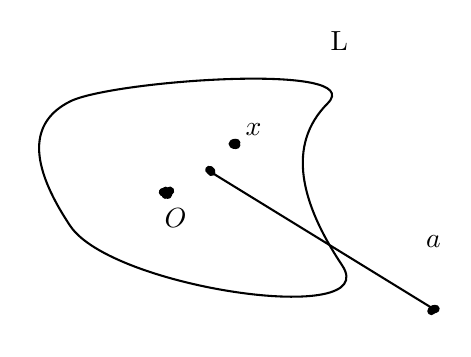
\begin{tikzpicture}[x=0.75pt,y=0.75pt,yscale=-1,xscale=1]
%uncomment if require: \path (0,300); %set diagram left start at 0, and has height of 300

%Shape: Polygon Curved [id:ds7874613059025218] 
\draw   (275,128) .. controls (295,118) and (419,109) .. (399,129) .. controls (379,149) and (386,177) .. (406,207) .. controls (426,237) and (295,218) .. (275,188) .. controls (255,158) and (255,138) .. (275,128) -- cycle ;
%Shape: Free Drawing [id:dp7812600627651304] 
\draw  [color={rgb, 255:red, 0; green, 0; blue, 0 }  ][line width=3] [line join = round][line cap = round] (321,172) .. controls (321,170.11) and (321,171.11) .. (321,173) .. controls (321,173.53) and (322,169.1) .. (322,173) .. controls (322,173.75) and (322.25,171) .. (323,171) .. controls (324.05,171) and (321,172.33) .. (320,172) .. controls (317.97,171.32) and (323.91,172) .. (320,172) ;
%Shape: Free Drawing [id:dp8115363247990739] 
\draw  [color={rgb, 255:red, 0; green, 0; blue, 0 }  ][line width=3] [line join = round][line cap = round] (355,149) .. controls (352.67,149) and (352.67,148) .. (355,148) ;
%Shape: Free Drawing [id:dp27311572912215587] 
\draw  [color={rgb, 255:red, 0; green, 0; blue, 0 }  ][line width=3] [line join = round][line cap = round] (342,161) .. controls (342.47,161) and (343,161.53) .. (343,162) ;
%Shape: Free Drawing [id:dp2686631289340635] 
\draw  [color={rgb, 255:red, 0; green, 0; blue, 0 }  ][line width=3] [line join = round][line cap = round] (449,229) .. controls (449,228.25) and (450.25,228) .. (451,228) ;
%Straight Lines [id:da31241161349044844] 
\draw    (341,161) -- (450,228) ;

% Text Node
\draw (358,137.4) node [anchor=north west][inner sep=0.75pt]    {$x$};
% Text Node
\draw (399,93) node [anchor=north west][inner sep=0.75pt]   [align=left] {L};
% Text Node
\draw (319,178.4) node [anchor=north west][inner sep=0.75pt]    {$O$};
% Text Node
\draw (445,191.4) node [anchor=north west][inner sep=0.75pt]    {$a$};


\end{tikzpicture}

\begin{statement}
    $x^* $ --- точка минимума $\hence x^* - a \perp l \forall l \in L \Longleftrightarrow \langle x^* - a , l \rangle = 0 $ 
\end{statement}

\begin{proof}
    \[ 
        0 = \frac{\partial f}{\partial l}(x^*) = \lim_{t \to 0} \frac{f^2(x^* + tl) - f^2(x^*)}{t} = \lim_{t \to 0} \frac{\langle x^* - a + tl, x^* - a + tl \rangle - \langle x^* - a, x^ * - a}{t}  = 2 Re \langle l, x ^ * - a \rangle
    \]
\end{proof}

\end{example}


\begin{exercise}
    Если $L$ замкнуто $\hence$ минимум существует
\end{exercise}

